\chapter{Evaluation} \label{chp:Evaluation}
In this chapter we want to present and discuss our evaluation results. Using Baselines Lab, we perform tests in a variety of different scenarios. After explaining our general test procedure in Section \ref{sec:TestProcedure}, we will begin, by evaluating the basic components for solving maze environments. In Section \ref{sec:EvalReward} we will take a look at reward generation and continue with a deeper look into observation generation and preprocessing in Section \ref{sec:EvalObs}. Section \ref{sec:EvalRLAlgorithms} will shine some light on the question which learning algorithm performs best when dealing with our particle navigation task and we will wrap up the evaluation of the basic parameters in Section \ref{sec:EvalParameters} where we take a look at the influence of various RL hyperparameters.

The initial tests will allow us to generate a baseline for the performance of our model, which then will be used throughout the rest of the evaluation to compare the influence of other factors. We begin, by testing how much inaccuracy in both actions and observations will influence the agent in Section \ref{sec:EvalError} and continue with the extension of the particle model with physical particles in Section \ref{sec:EvalPhysical}. We will then take a look at randomized instances in Section \ref{sec:EvalRandomness} and finish with a comparison with algorithmic approaches in Section \ref{sec:EvalAlgorithms}.


\section{Test Procedure} \label{sec:TestProcedure}
In this section we want to talk about different aspects of our test procedure.

\paragraph{Environment.}
All experiments were done on a Linux workstation running Ubuntu 18.04 LTS. The workstation has an Intel 6700K CPU, a single Nvidia GeForce GTX 1080 Ti GPU and 64GB of main memory. We installed Python 3.7.3 using the Anaconda \cite{anaconda} software distribution. We also used Tensorflow 1.14 in conjunction with the CUDA Toolkit version 10.1.243 and CUDNN version 7.6.5. Baselines Lab was developed on top of Stable-Baselines 2.10 and NumPy 1.17. For a complete list of installed packages see Appendix \ref{apx:BaselinesLab}.

\paragraph{Procedure.}
Our experiments involved several sources of randomness. To ensure consistent executions, we fixed the random seed for all involved components to the same value for all experiments. Unfortunately Tensorflow 1.14 does not guarantee consistent results during GPU computations. We therefore repeated experiments three times and averaged the results for comparison. The learning curves provided in this chapter are also smoothed by an exponential weighted moving average, using a factor of $0.6$.

To determine the performance of a configuration, we look at the end result during training for the average and best trial. We also determine the step in which the average episode length becomes smaller by five percent in comparison to the environments' time limit. We call this moment the \textit{drop}, since performance usually suddenly increases when the agent is able to reach the goal for the first time. The drop can be used as an indicator for how fast the agent is able to find a first usable result, while the end-of-training episode length is an indicator for how good the best solution is the agent is able to find. 

\paragraph{Initial Hyperparameters.}
For our initial experiments we wanted to use general purpose hyperparameters for the PPO algorithm. We therefore used parameters similar to the parameters used in the RND paper \cite{burda2018exploration} (see Table \ref{tab:RNDParameters}) which showed to produce good results across all Atari environments. 


\begin{table} [ht]
    \begin{center}
        \begin{tabular}{|c|c|}
            \hline
            Hyperparameter & Value \\
            \hline
            Rollout Length & 256 \\
            Number of minibatches & 8 \\
            Number of optimization epochs & 16 \\
            Number of parallel environments & 64 \\
            Learning rate & 0.0001 \\
            Optimization algorithm & Adam \cite{kingma2014adam} \\
            $\lambda$ & 0.95 \\
            Entropy coefficient & 0.001 \\
            $\gamma$ & 0.99 \\
            Clip range & [0.9, 1.1] \\
            \hline
        \end{tabular}
    \end{center}
    \caption[Default Hyperparameters]{Default hyperparameters for PPO for the initial experiments.} \label{tab:RNDParameters}
\end{table}

We also used a common preprocessing pipeline for the observations which was also used by Huang et al.:

\begin{table} [h]
    \begin{center}
        \begin{tabular}{|c|c|}
            \hline
            Hyperparameter & Value \\
            \hline
            Observation downsampling & (84, 84) \\
            Max steps per episode & 2000 \\
            Max and skip Frames & 4 \\
            Frame stacking & 4 \\
            \hline
        \end{tabular}
    \end{center}
    \caption[Default Observation Preprocessing]{Default observation preprocessing for all environments.} \label{tab:RNDParameters}
\end{table}

If not stated otherwise, we also normalized the observations by $x \mapsto x/255$. Observations for the RND curiosity module are normalized by $x \mapsto CLIP((x-\mu)/\sigma, [-5, 5])$ instead and no frame stacking is applied.


\paragraph{Instances.}
To allow easy comparison, we used the same instances as in previous work for our experiments. We included a description of these instances in Table \ref{tab:TestInstances}. Previous work showed, that these instances provide a good scale of difficulty between easy (\texttt{Corridor}) and hard (\texttt{Brain}). Instances with less paths to the goal position seem to be harder to solve, since they require more precise manoeuvering instead of just pulling all particles into a general direction. To increase the difficulty of our medium instance, we therefore replaced it with an instance generated by our RRT instance generator. This instance can also be seen in Table \ref{tab:TestInstances} and is called \texttt{Vessel}. The Vessel maze has similar dimensions in comparison with Corridor, but has far more fine grained structures where particles may have collisions. There is also only a single path to the goal position. Additionally the Vessel maze covers a large part of the input, allowing for a lot more possible states than Corridor. 

% \begin{table} [h!]
%     \begin{center}
%         \begin{tabular}{|c|c|c|c|c|c|}
%             \hline
%             Instance & Name & Dimension & Size (\% of Area) & $d_{avg}$ & $d_{max}$ \\
%             \hline
%             &&&&&\\[-1em]
%             \parbox[c]{3.5cm}{
\includegraphics[clip, width=3.5cm]{figures/evaluation/procedure/corridor_upscaled.png}} & Corridor & $(100 \times 100)$ & $2869 \ (= 28.69\%)$ & 73.65 & 117 \\
%             &&&&&\\[-1em]
%             \hline
%             &&&&&\\[-1em]
%             \parbox[c]{3.5cm}{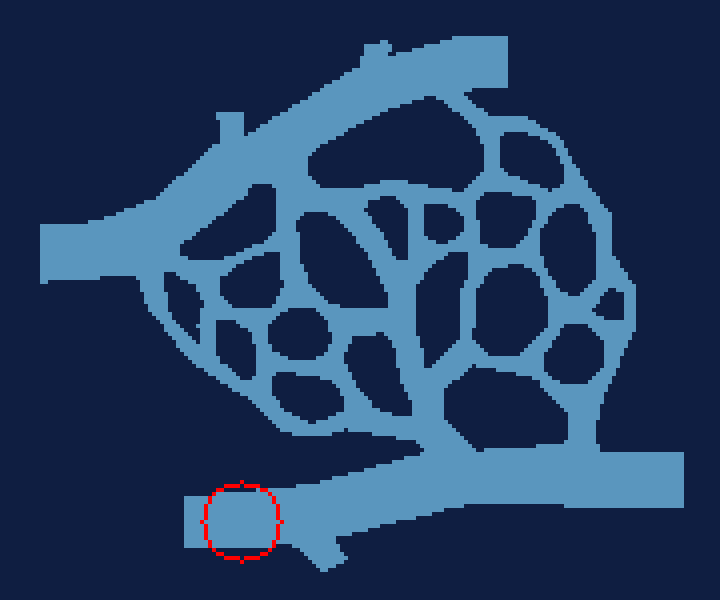
\includegraphics[clip, width=3.5cm]{figures/evaluation/procedure/capillary_upscaled.png}} & Capillary & $(180 \times 150)$ & $7169 \ (\approx 26.55\%)$ & 91.22 & 149 \\
%             &&&&&\\[-1em]
%             \hline
%             &&&&&\\[-1em]
%             \parbox[c]{3.5cm}{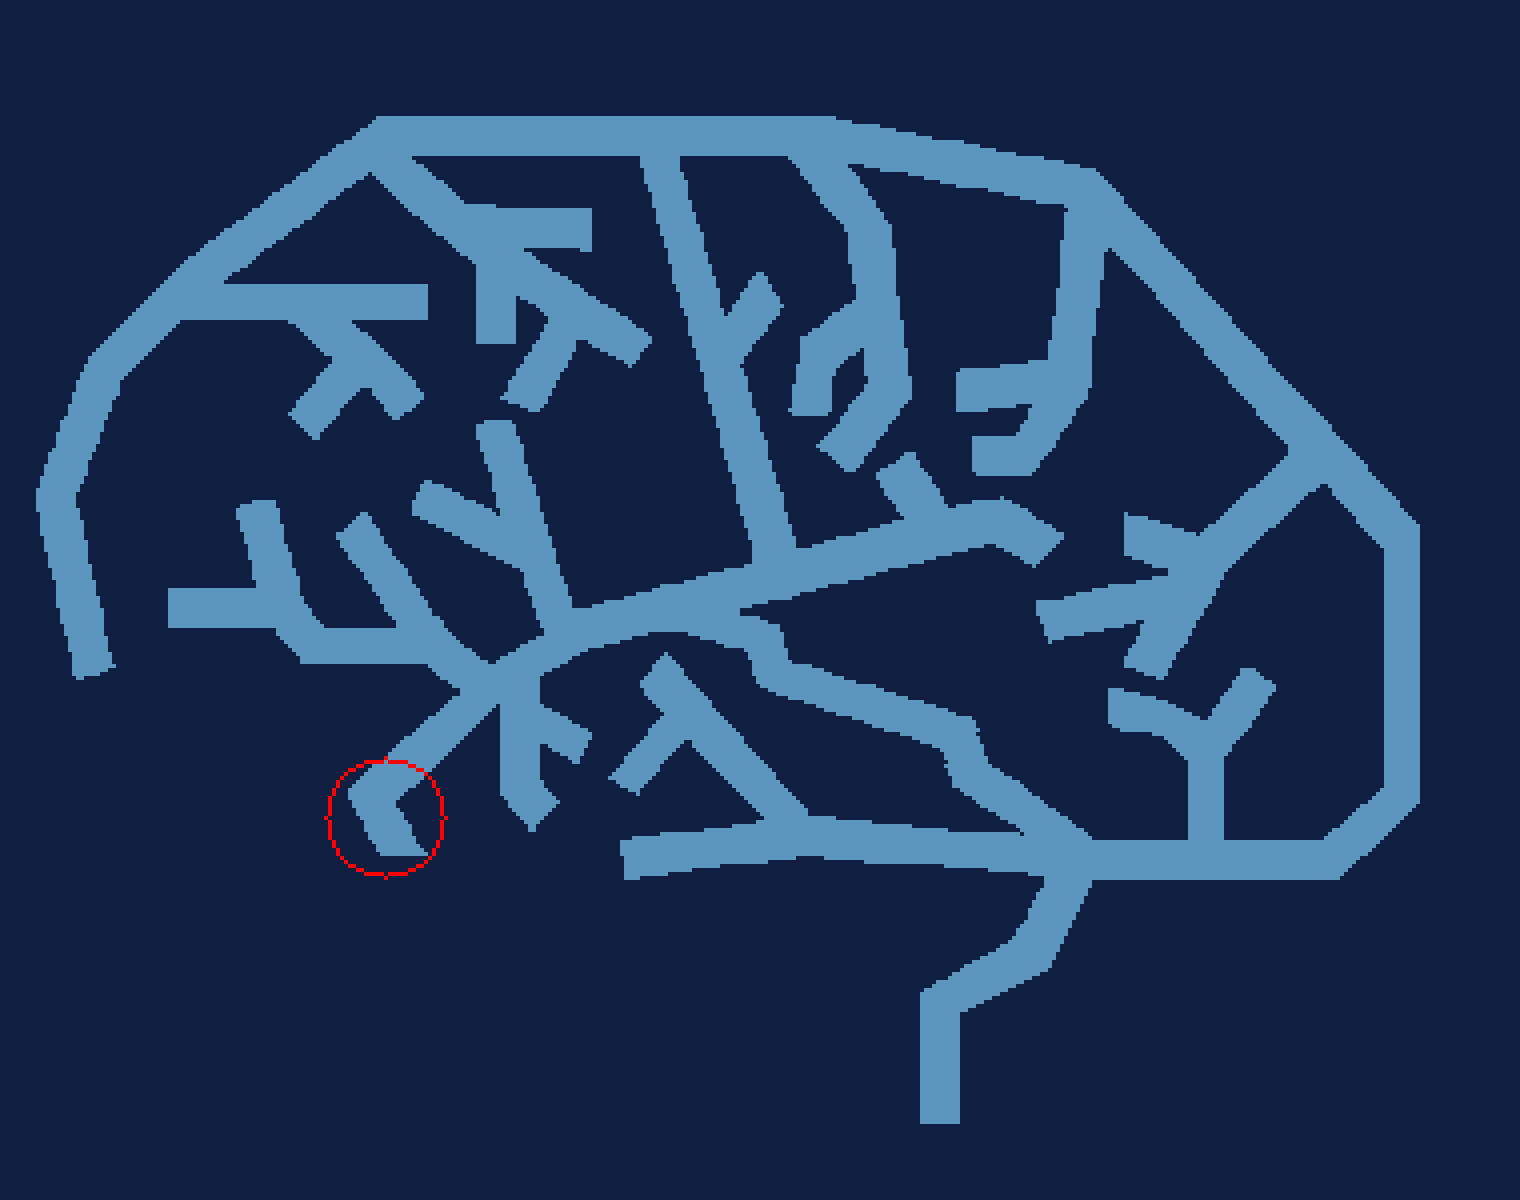
\includegraphics[clip, width=3.5cm]{figures/evaluation/procedure/brain_upscaled.png}} & Brain & $(380 \times 300)$ & $22593 \ (\approx 19.82\%)$ & 221.19 & 400 \\
%             &&&&&\\[-1em]
%             \hline
%             &&&&&\\[-1em]
%             \parbox[c]{3.5cm}{
\includegraphics[clip, width=3.5cm]{figures/evaluation/procedure/vessel_upscaled.png}} & Vessel & $(130 \times 80)$ & $4949 \ (\approx 47.59\%)$ & 77.47 & 136 \\[1cm]
%             \hline
%         \end{tabular}
%     \end{center}
%     \caption[Test Instances]{A list of our default test instances. Light blue pixels denote non-blocked pixels. The goal position is marked with a red circle. \textit{Dimension} describes the absolute size of the instance, while \textit{size} denotes the actual non-blocked area. We also included values for the average $d_{avg}$ and maximum $d_{max}$ distance between any point and the goal position.} \label{tab:TestInstances}
% \end{table}

\begin{table} [h!]
    \begin{center}
        \begin{tabular}{cccccc}
            \toprule
            Instance & Name & Dimension & Size (\% of Area) & $d_{avg}$ & $d_{max}$ \\
            \midrule
            
            \parbox[c]{3.5cm}{
\includegraphics[clip, width=3.5cm]{figures/evaluation/procedure/corridor_upscaled.png}} & Corridor & $(100 \times 100)$ & $2869 \ (= 28.69\%)$ & 73.65 & 117 \\
            \addlinespace[0.05cm]
            \midrule
            
            \parbox[c]{3.5cm}{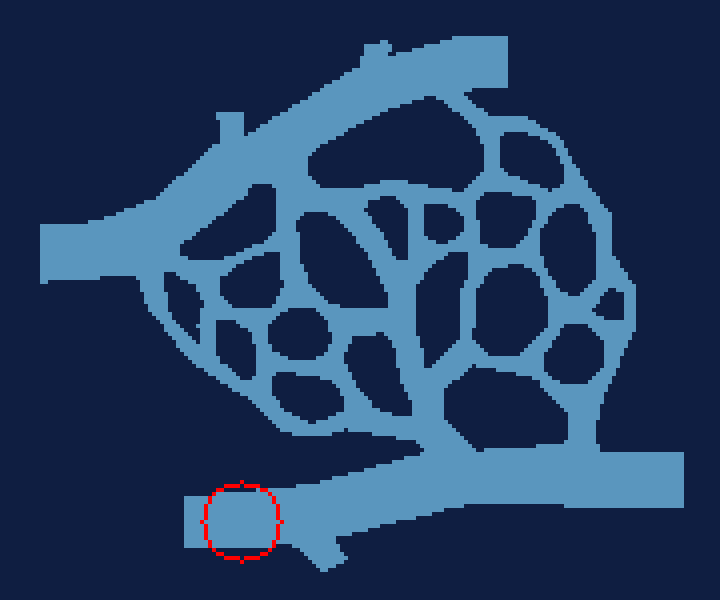
\includegraphics[clip, width=3.5cm]{figures/evaluation/procedure/capillary_upscaled.png}} & Capillary & $(180 \times 150)$ & $7169 \ (\approx 26.55\%)$ & 91.22 & 149 \\
            \addlinespace[0.05cm]
            \midrule
            
            \parbox[c]{3.5cm}{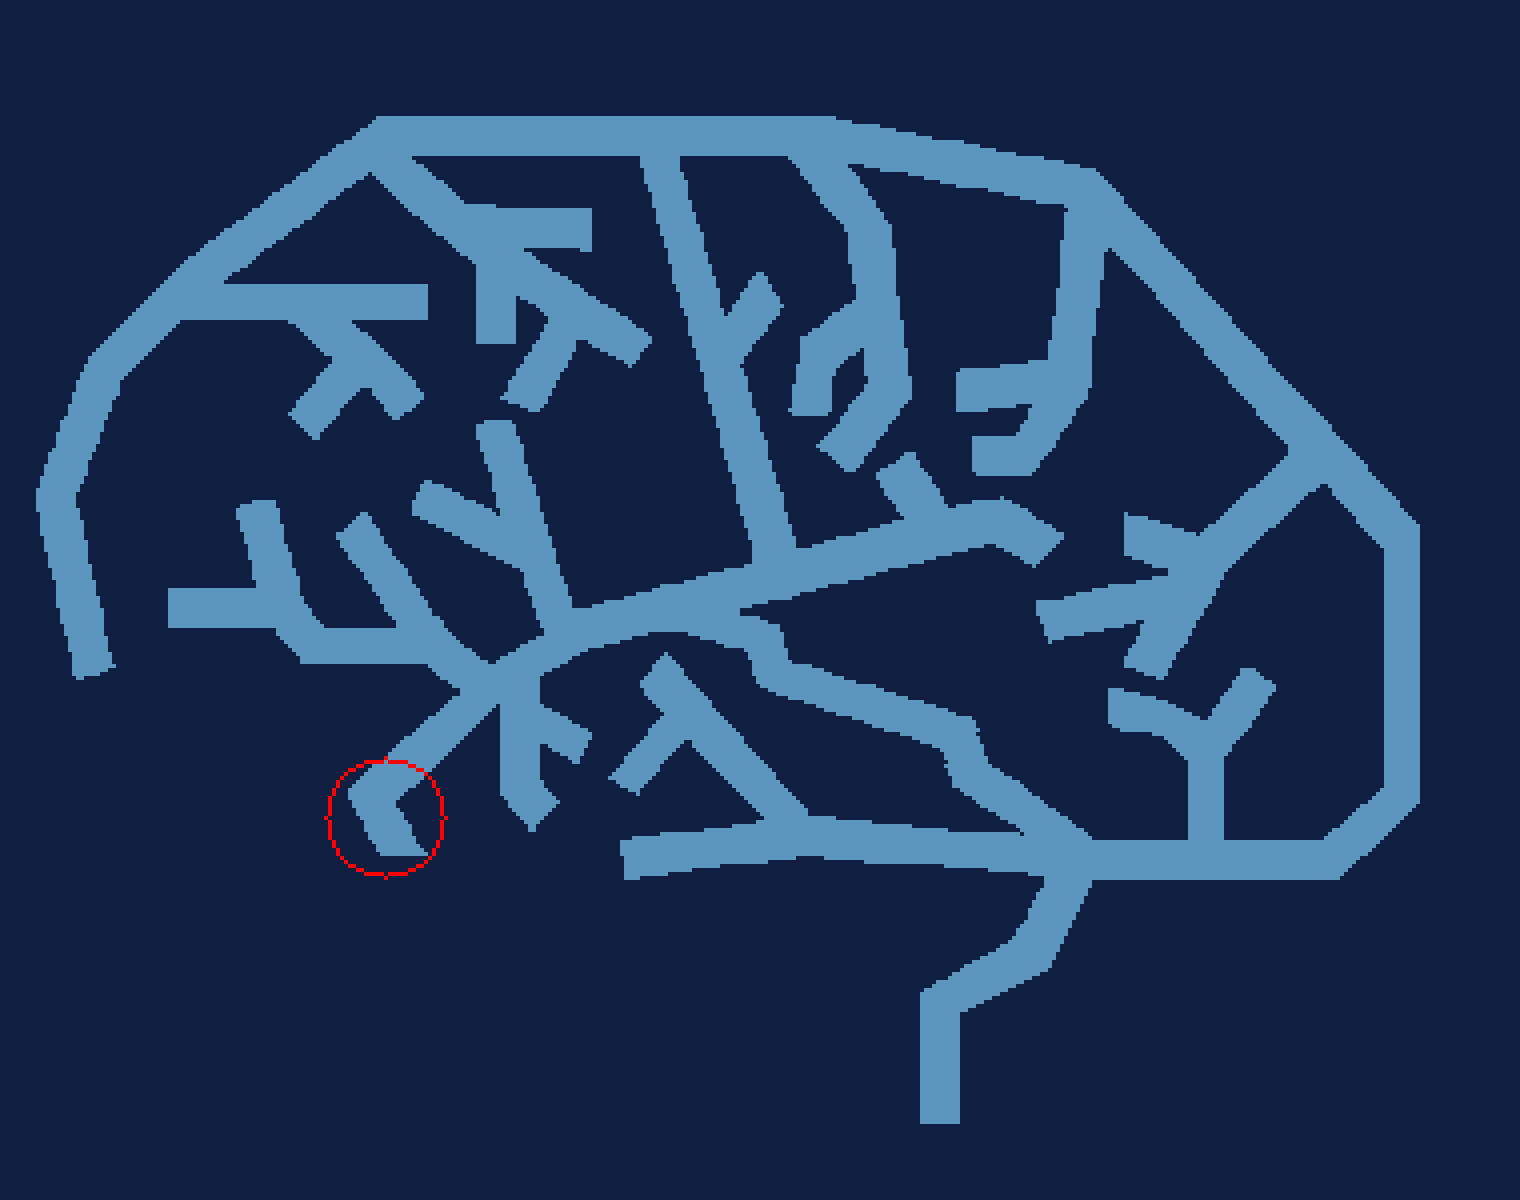
\includegraphics[clip, width=3.5cm]{figures/evaluation/procedure/brain_upscaled.png}} & Brain & $(380 \times 300)$ & $22593 \ (\approx 19.82\%)$ & 221.19 & 400 \\
            \addlinespace[0.05cm]
            \midrule
            
            \parbox[c]{3.5cm}{
\includegraphics[clip, width=3.5cm]{figures/evaluation/procedure/vessel_upscaled.png}} & Vessel & $(130 \times 80)$ & $4949 \ (\approx 47.59\%)$ & 77.47 & 136 \\
            \addlinespace[0.05cm]
            \bottomrule
        \end{tabular}
    \end{center}
    \caption[Test Instances]{A list of our default test instances. Light blue pixels denote non-blocked pixels. The goal position is marked with a red circle. \textit{Dimension} describes the absolute size of the instance, while \textit{size} denotes the actual non-blocked area. We also included values for the average $d_{avg}$ and maximum $d_{max}$ distance between any point and the goal position.} \label{tab:TestInstances}
\end{table}

If not stated otherwise, we used 256 randomly generated particles for each episode during training. Instances are capped at a maximum of 2000 steps per episode independent of the use of dynamic episode length.

\section{Reward Generation} \label{sec:EvalReward}
We begin our experiments by analyzing which reward works best to guide particles to the goal position. We expect that different rewards will heavily impact training performance and will therefore be very important for later experiments. Since we are dealing with a huge number of possible combinations in our reward system, we decide to use an iterative approach: We first test many combinations on the easy Corridor instance and then only evaluate the promising combinations on the Vessel instance. We finally select only the best performing combinations from the Vessel instance and test them on the Brain instance. Since observation normalization can have a huge impact on training performance and directly influences reward generation in the case of intrinsic reward, we also decided to add observation normalization in the form of $x \mapsto CLIP((x - \mu)/\sigma, [-10, 10])$ into this experiment.

Throughout this section we will provide a number of tables, which use abbreviations to save space. The abbreviations are explained in Table \ref{tab:RewardAbbreviations}.  

\begin{table} [ht]
    \begin{center}
        \begin{tabular}{ll}
            \toprule
            \multicolumn{1}{c}{Reward Component} & Abbreviation \\
            \midrule
            Continuous Reward & CR \\
            Discrete Reward & DR \\
            Observation Normalization & ON \\
            Reward Normalization & RN \\
            Time Penalty & TP \\
            Dynamic Episode Length & DEL \\
            Curiosity Reward & RND \\
            Gathering Reward & GR \\
            \bottomrule
            
        \end{tabular}
    \end{center}
    \caption[Abbreviations for Reward Components]{Common abbreviations for reward components} \label{tab:RewardAbbreviations}
\end{table}



\paragraph{Corridor Environemnt.}
We begin with our easy instance Corridor. In our tests, we use the basic settings from Section \ref{sec:TestProcedure} and train for 3 million steps per trial. Table \ref{tab:Maze0318/Reward/Discrete} contains the results for discrete rewards and Table \ref{tab:Maze0318/Reward/Continuous} contains the results for continuous rewards.

Looking at the data, we can see, that many parameters do work very well and our dense discrete reward produces results which result in vastly shorter training times than the previous reward of Huang et al. \cite{huang2019}. Our initial experiments for discrete reward also show some interesting findings: 
\begin{itemize}
    \item \textbf{Normalization. } We found, that normalization has a huge impact on training performance. Normalization the reward has a positive impact on its own (see Experiments 4/6), but additionally normalizing the observation seems to be very important to improve performance (see Experiments 7/11 or 8/10).
    \item \textbf{Curiosity. } Using our relatively dense discrete reward, curiosity does not seem to have a positive effect for simple instances. Using DEL, a small amount of curiosity reward seems to have a positive impact (see Experiments 1/3), but also can have a negative impact if the weight is higher (see Experiments 1/2 or 13/14). Curiosity may have a greater impact when training with more complex instances though.
    \item \textbf{Dynamic Episode Length. } DEL does not seem to have any positive impact on the training performance. Experiment 9 shows that DEL is capable of creating time penalty like pressure, but the final result is worse than training with our normal time penalty. In combination with curiosity reward or a standard time penalty, performance seems to also worsen. (see Experiments 11/13; 12/14)
    \item \textbf{Gathering Reward. } Gathering reward does not seem to have any influence on the performance for small instances. Further testing will show, if this changes with larger or more challenging instances, where gathering of particles before bringing them to the goal might be more beneficial.
\end{itemize}


\begin{table}[htp]
    \begin{center}
        \begin{tabular}{rccccccrrr}
            \toprule
             & \multicolumn{6}{c}{Reward Component} & \multicolumn{2}{c}{Episode Length} & \\
            \cmidrule(lr){2-7}\cmidrule(lr){8-9}
            \multicolumn{1}{c}{Idx} & \multicolumn{1}{c}{ON} & \multicolumn{1}{c}{RN} & \multicolumn{1}{c}{TP} & \multicolumn{1}{c}{DEL} & \multicolumn{1}{c}{RND} & \multicolumn{1}{c}{GR} & \multicolumn{1}{c}{Best} & \multicolumn{1}{c}{Avg} & \multicolumn{1}{c}{Drop}\\
            \midrule
            1 &  &  &  & X &  &  & 256.78 & 295.04 & 1.25M \\
            2 &  &  &  & X & 0.50 &  & 499.97 & 499.99 & 750k \\
            3 &  &  &  & X & 0.25 &  & 110.94 & 117.82 & 750k \\
            4 &  &  & X &  &  &  & 135.03 & 145.34 & 629k \\
            5 &  &  & X &  & 0.25 &  & 324.29 & 422.48 & 456k \\
            6 &  &  & X & X &  &  & 477.62 & 491.48 & 3M \\
            7 &  & X & X &  &  &  & 83.78 & 84.66 & 461k \\
            8 &  & X & X &  &  & 1.00 & 93.31 & 94.30 & 406k \\
            9 & X & X &  & X &  &  & 65.72 & 67.17 & 400k \\
            10 & X & X & X &  &  & 1.00 & 59.31 & \textbf{65.68} & 190k \\
            11 & X & X & X &  &  &  & \textbf{57.38} & 66.81 & 182k \\
            12 & X & X & X &  & 0.50 &  & 84.52 & 207.78 & \textbf{181k} \\
            13 & X & X & X & X &  &  & 65.34 & 78.93 & 400k \\
            14 & X & X & X & X & 0.50 &  & 500.00 & 500.00 & 3M \\
            \bottomrule
        \end{tabular}
    \end{center}
    \caption[Evaluation of Discrete Reward Evaluation with the Corridor Environment]{Evaluation of discrete rewards with the corridor environment.} \label{tab:Maze0318/Reward/Discrete}
\end{table}


The evaluation results using continuous reward show similar outcomes to the experiments using discrete reward. The most important finding is, that the best continuous reward is able to produce superior results in every category compared to the best discrete reward. Especially the time of first notable improvement is about 30\% earlier. We included a plot showing the average episode length during training in Figure \ref{fig:ContinuousVsDiscrete}. This further supports our decision to create more dense rewards. 

\begin{table}[htp]
    \begin{center}
        \begin{tabular}{rccccccccrrr}
            \toprule
             & \multicolumn{8}{c}{Reward Component} & \multicolumn{2}{c}{Episode Length} & \\
            \cmidrule(lr){2-9}\cmidrule(lr){10-11}
            \multicolumn{1}{c}{Idx} & \multicolumn{1}{c}{ON} & \multicolumn{1}{c}{RN} & \multicolumn{1}{c}{TP} & \multicolumn{1}{c}{DEL} & \multicolumn{1}{c}{RND} & \multicolumn{1}{c}{GR} & \multicolumn{1}{c}{Int Norm} & \multicolumn{1}{c}{PO} & \multicolumn{1}{c}{Best} & \multicolumn{1}{c}{Avg} & \multicolumn{1}{c}{Drop}\\
            \midrule
            1 &  &  &  & X &  &  & X &  & 101.06 & 106.07 & 600k \\
            2 &  &  &  & X & 0.25 &  & X &  & 394.12 & 413.82 & 800k \\
            3 &  &  & X &  &  &  &  &  & 146.38 & 149.47 & 787k \\
            4 &  &  & X &  &  &  & X &  & 102.44 & 103.96 & 718k \\
            5 &  &  & X & X &  &  & X &  & 92.12 & 96.00 & 400k \\
            6 &  & X & X &  &  &  & X & X & 90.47 & 98.18 & 370k \\
            7 &  & X & X &  &  &  & X &  & 101.62 & 102.40 & 525k \\
            8 &  & X & X &  &  & 1.00 & X &  & 96.22 & 103.99 & 614k \\
            9 &  & X & X &  & 0.25 &  & X &  & 198.44 & 335.29 & 561k \\
            10 & X & X &  & X &  &  & X &  & 82.41 & 83.32 & 400k \\
            11 & X & X & X &  &  &  &  &  & \textbf{56.59} & \textbf{59.04} & \textbf{127k} \\
            12 & X & X & X &  &  &  & X & X & 58.72 & 65.46 & 152k \\
            13 & X & X & X &  &  &  & X &  & 61.81 & 71.28 & 147k \\
            14 & X & X & X &  &  & 1.00 &  &  & 60.53 & 62.46 & 149k \\
            15 & X & X & X &  &  & 1.00 & X &  & 59.09 & 68.69 & 151k \\
            16 & X & X & X &  & 0.25 &  & X & X & 69.41 & 246.38 & 158k \\
            17 & X & X & X & X &  &  & X & X & 79.19 & 79.39 & 400k \\
            \bottomrule
        \end{tabular}
    \end{center}
    \caption[Evaluation of Continuous Reward with the Corridor Environment]{Evaluation of continuous rewards with the corridor environment.} \label{tab:Maze0318/Reward/Continuous}
\end{table}


\begin{figure}[htp]
    
    \begin{center}
        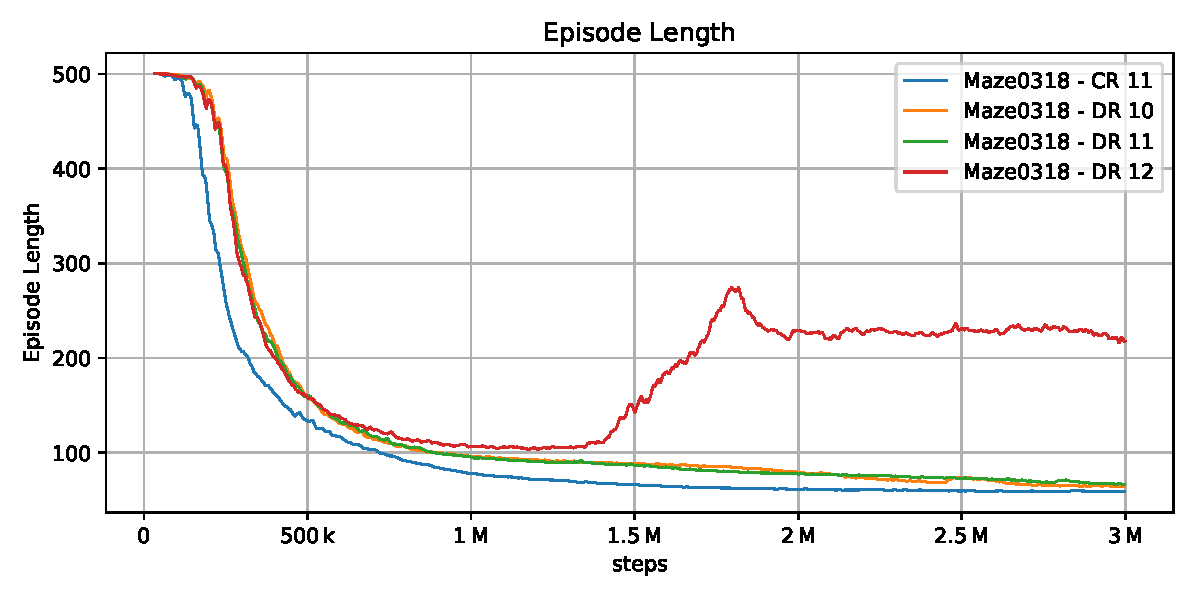
\includegraphics[clip, width=0.75\columnwidth]{figures/evaluation/rewards/continuous_vs_discrete.pdf}
    \end{center}
    
    %\vspace*{-6pt}
    \caption[Training Curves with Curiosity Reward]{Average episode length on the corridor environment during training. The legend refers to experiment numbers.}
    \label{fig:ContinuousVsDiscrete}
    %\vspace*{-12pt}
\end{figure}

\begin{figure}[htp]
    
    \begin{center}
        \begin{tabular}{c}
            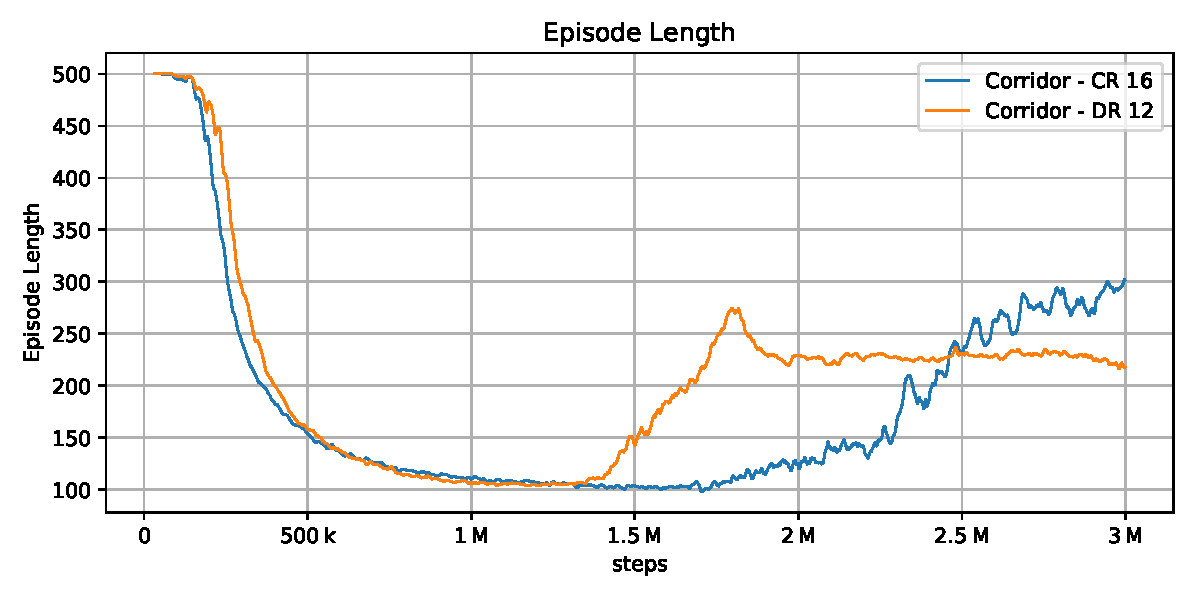
\includegraphics[clip, width=0.75\columnwidth]{figures/evaluation/rewards/curiosity_divergence_ep_len.pdf} \\
            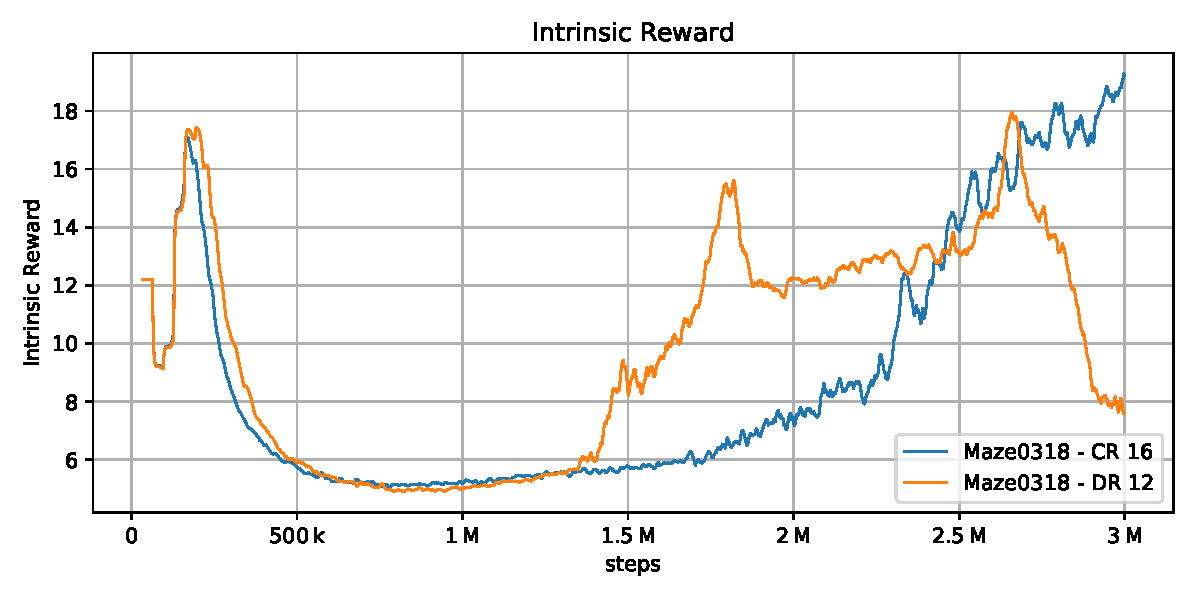
\includegraphics[clip, width=0.75\columnwidth]{figures/evaluation/rewards/curiosity_divergence_int_rew.pdf} \\
            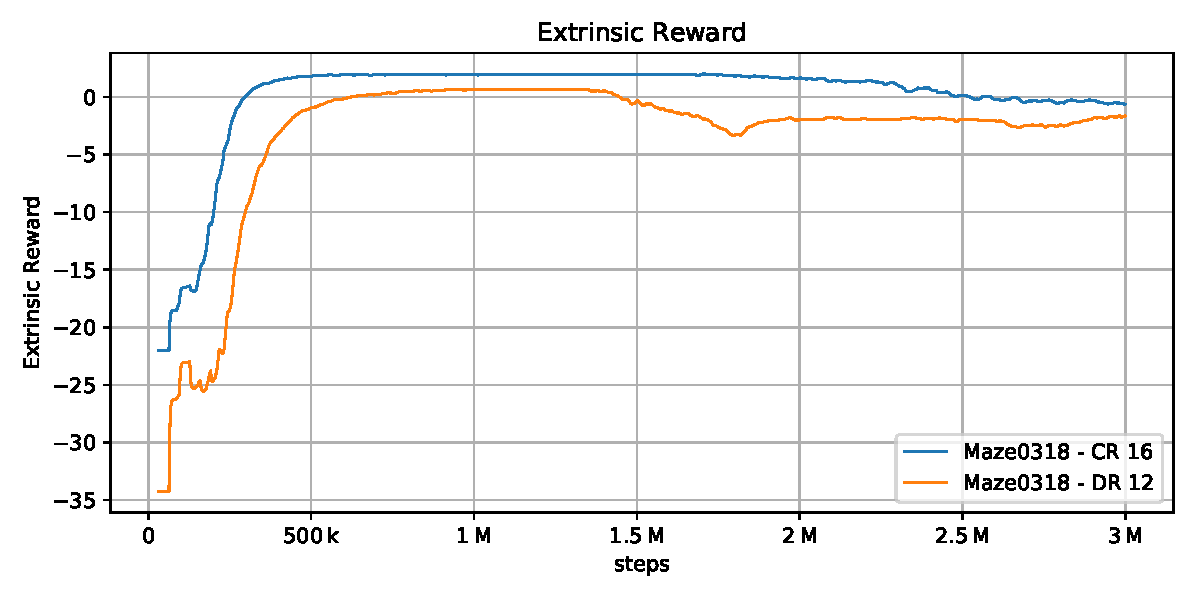
\includegraphics[clip, width=0.75\columnwidth]{figures/evaluation/rewards/curiosity_divergence_ext_rew.pdf}
        \end{tabular}

    \end{center}
    
    %\vspace*{-6pt}
    \caption[Problems with Curiosity Reward]{Learning curves for training with curiosity reward. We observed, that often intrinsic rewards tends to take over and result in a performance collapse during training at some point. This can be seen, by comparing the intrinsic to the extrinsic reward and looking at the episode length: At around 1.5 million training steps, the intrinsic reward begins to increase, while the extrinsic reward stays at a constant value. At the same time, the average episode length begins to increase.}
    \label{fig:CuriosityDiverge}
    %\vspace*{-12pt}
\end{figure}


Similar to the results obtained when using discrete rewards, we can see, that normalization massively improves performance for continuous rewards. Curiosity also does not seem to improve the results and often tends to diverge from the optimum at the end of training as shown in Figure \ref{fig:CuriosityDiverge}. Otherwise the corridor instance seems to be too easy to show differences between other reward parameters. Like before, gathering reward does not seem to have any positive or negative impact. The use of positive only rewards shows to improve performance without normalization (see Experiments 3/4), but only has a small impact with normalization (see Experiments 12/13). Interestingly internal normalization which balances the total cost reward against the maximum cost reward has shown to worsen the results on the corridor environment (see Experiments 11/13). 


\paragraph{Vessel Environment.} We repeat multiple experiments on the more complicated, but similarly large vessel instance. The results for discrete rewards are shown in Table \ref{tab:VesselMaze02/Reward/Discrete} and the results for continuous reward in Table \ref{tab:VesselMaze02/Reward/Continuous}. To compensate for the more complex environment, we double the training time for the agent and train for 6 millions steps per trial. 

Looking at the results for discrete rewards in Table \ref{tab:VesselMaze02/Reward/Discrete}, we can see, that normalization is crucial for success. While agents trained with non-normalized rewards are still able to find solutions, they need much more training time. For discrete rewards, the addition of an supporting reward signals seems to be important: The experiments including dynamic episode length (3), gathering reward (5) or curiosity reward (6) all produced better results, than stand-alone discrete reward (4). Especially the combination of discrete reward with curiosity was able to find a solution in a relatively short time. Note, that training with curiosity is significantly slower due to the extra computation for the training of the predictor network. 

\begin{table}[htp]
    \begin{center}
        \begin{tabular}{rccccccrrr}
            \toprule
             & \multicolumn{6}{c}{Reward Component} & \multicolumn{2}{c}{Episode Length} & \\
            \cmidrule(lr){2-7}\cmidrule(lr){8-9}
            \multicolumn{1}{c}{Idx} & \multicolumn{1}{c}{ON} & \multicolumn{1}{c}{RN} & \multicolumn{1}{c}{TP} & \multicolumn{1}{c}{DEL} & \multicolumn{1}{c}{RND} & \multicolumn{1}{c}{GR} & \multicolumn{1}{c}{Best} & \multicolumn{1}{c}{Avg} & \multicolumn{1}{c}{Drop}\\
            \midrule
            1 &  &  &  & X & 0.25 &  & 478.91 & 487.95 & 9.99M \\
            2 &  &  & X &  & 0.25 &  & 491.19 & 497.06 & 9.99M \\
            3 & X & X &  & X &  &  & \textbf{89.38} & 95.75 & 1.2M \\
            4 & X & X & X &  &  &  & 97.28 & 100.09 & 762k \\
            5 & X & X & X &  &  & 1.00 & 93.78 & \textbf{95.15} & 828k \\
            6 & X & X & X &  & 0.50 &  & 107.31 & 109.18 & \textbf{694k} \\
            7 & X & X & X & X &  &  & 89.62 & 96.38 & 1.2M \\
            \bottomrule
        \end{tabular}
    \end{center}
    \caption[Evaluation of Discrete Reward Evaluation with the Vessel Environment]{Evaluation of discrete rewards with the vessel environment.} \label{tab:VesselMaze02/Reward/Discrete}
\end{table}


The results for continuous rewards differ from the results for discrete rewards. By looking at Table \ref{tab:VesselMaze02/Reward/Continuous} we can see, that the addition of supporting rewards often produces worse results (see Experiments 7/11, 4/5, 8/10). An exception seems to be the combination of gathering reward with not internally normalized reward (see Experiments 6/9). Using only positive reward, does not seem to improve performance. The same is true for dynamic episode lengths.  


\begin{table}[htp]
    \begin{center}
        \begin{tabular}{rccccccccrrr}
            \toprule
             & \multicolumn{8}{c}{Reward Component} & \multicolumn{2}{c}{Episode Length} & \\
            \cmidrule(lr){2-9}\cmidrule(lr){10-11}
            \multicolumn{1}{c}{Idx} & \multicolumn{1}{c}{ON} & \multicolumn{1}{c}{RN} & \multicolumn{1}{c}{TP} & \multicolumn{1}{c}{DEL} & \multicolumn{1}{c}{RND} & \multicolumn{1}{c}{GR} & \multicolumn{1}{c}{Int Norm} & \multicolumn{1}{c}{PO} & \multicolumn{1}{c}{Best} & \multicolumn{1}{c}{Avg} & \multicolumn{1}{c}{Drop}\\
            \midrule
            1 &  &  & X &  & 0.25 &  & X &  & 451.00 & 476.26 & 7.92M \\
            2 &  & X & X &  &  &  &  &  & 423.09 & 433.16 & 7.81M \\
            3 &  & X & X &  &  &  & X & X & 373.28 & 405.12 & 8M \\
            4 &  & X & X &  &  &  & X &  & 416.28 & 458.89 & 7.91M \\
            5 &  & X & X &  &  & 1.00 & X &  & 418.75 & 470.94 & 7.05M \\
            6 & X & X & X &  &  &  &  &  & 93.97 & 98.73 & \textbf{501k} \\
            7 & X & X & X &  &  &  & X & X & 103.16 & 105.57 & 628k \\
            8 & X & X & X &  &  &  & X &  & 91.06 & \textbf{96.72} & 532k \\
            9 & X & X & X &  &  & 1.00 &  &  & \textbf{89.41} & 100.26 & 600k \\
            10 & X & X & X &  &  & 1.00 & X &  & 95.16 & 98.65 & 507k \\
            11 & X & X & X &  & 0.25 &  & X & X & 126.94 & 197.88 & 601k \\
            12 & X & X & X & X &  &  & X & X & 185.62 & 193.65 & 2.8M \\
            \bottomrule
        \end{tabular}
    \end{center}
    \caption[Evaluation of Continuous Reward with the Vessel Environment]{Evaluation of continuous rewards with the vessel environment.} \label{tab:VesselMaze02/Reward/Continuous}
\end{table}

\paragraph{Brain Environment.} We finally tested our the best performing reward configurations from the vessel environment on the brain environment. To compensate for the larger instance size and increased complexity, we again doubled training times, resulting in a total of 12 million training steps per trial. 

The results for discrete reward are listed in Table \ref{tab:Maze0122/Reward/Discrete}. Surprisingly, two of the three selected rewards did perform very poorly. Neither the configuration with dynamic episode length nor the one with curiosity reward did yield acceptable end results after 12 million training steps. The only discrete reward variation that can solve the brain environment successfully under the given time limit uses additional gathering reward. 


\begin{table}[htp]
    \begin{center}
        \begin{tabular}{rccccccrrr}
            \toprule
             & \multicolumn{6}{c}{Reward Component} & \multicolumn{2}{c}{Episode Length} & \\
            \cmidrule(lr){2-7}\cmidrule(lr){8-9}
            \multicolumn{1}{c}{Idx} & \multicolumn{1}{c}{ON} & \multicolumn{1}{c}{RN} & \multicolumn{1}{c}{TP} & \multicolumn{1}{c}{DEL} & \multicolumn{1}{c}{RND} & \multicolumn{1}{c}{GR} & \multicolumn{1}{c}{Best} & \multicolumn{1}{c}{Avg} & \multicolumn{1}{c}{Drop}\\
            \midrule
            1 & X & X &  & X &  &  & 500.00 & 500.00 & 12M \\
            2 & X & X & X &  &  & 1.00 & \textbf{311.44} & \textbf{319.23} & \textbf{7.15M} \\
            3 & X & X & X &  & 0.50 &  & 479.59 & 486.36 & 12M \\
            \bottomrule
        \end{tabular}
    \end{center}
    \caption[Evaluation of Discrete Reward with the Brain Environment]{Evaluation of discrete rewards with the brain environment.} \label{tab:Maze0122/Reward/Discrete}
\end{table}

In contrast to the discrete reward variations, all continuous reward configurations were able to solve the brain environment. As we can see from Table \ref{tab:Maze0122/Reward/Continuous}, the addition of gathering reward yields the best results, while internally normalized (balanced) continuous reward performs better than non-balanced reward.

\begin{table}[htp]
    \begin{center}
        \begin{tabular}{rccccccccrrr}
            \toprule
             & \multicolumn{8}{c}{Reward Component} & \multicolumn{2}{c}{Episode Length} & \\
            \cmidrule(lr){2-9}\cmidrule(lr){10-11}
            \multicolumn{1}{c}{Idx} & \multicolumn{1}{c}{ON} & \multicolumn{1}{c}{RN} & \multicolumn{1}{c}{TP} & \multicolumn{1}{c}{DEL} & \multicolumn{1}{c}{RND} & \multicolumn{1}{c}{GR} & \multicolumn{1}{c}{Int Norm} & \multicolumn{1}{c}{PO} & \multicolumn{1}{c}{Best} & \multicolumn{1}{c}{Avg} & \multicolumn{1}{c}{Drop}\\
            \midrule
            1 & X & X & X &  &  &  &  &  & 328.97 & 352.97 & 7.46M \\
            2 & X & X & X &  &  &  & X &  & \textbf{308.31} & 333.53 & 7.34M \\
            3 & X & X & X &  &  & 1.00 & X &  & 324.78 & \textbf{333.35} & \textbf{6.75M} \\
            \bottomrule
        \end{tabular}
    \end{center}
    \caption[Evaluation of Continuous Reward with the Brain Environment]{Evaluation of continuous rewards with the brain environment.} \label{tab:Maze0122/Reward/Continuous}
\end{table}

\paragraph{Conclusion.} When deciding for a reward for our further experiments, we have to keep in mind, that every extra computation will be executed for each individual training step. The more reward components we use, the longer training will take. When comparing the results on the brain environment for continuous reward, we saw that the addition of gathering reward just slightly improves the average end result. If we look at the wall-clock time, trials using the gathering reward took 4:50h to complete, while trials using only the continuous reward took 4:20h. This means that with gathering reward, we saw an increase of about 11.5\% more time. Since discrete rewards only scale well with additional reward components we always have the same problem here. We therefore will use continuous internally normalized reward for all further experiments.

The reward experiments also showed, that deviations between repeated trials are very small, but increase with instance size. This can be observed, by comparing the best and average result among different trials over our three test instances.

\section{Observations} \label{sec:EvalObs}
Observations
\section{RL Algorithms} \label{sec:EvalRLAlgorithms}
RL Algorithms
\section{Hyperparameters} \label{sec:EvalParameters}
Hyperparameters
\section{Extended Environment Models} \label{sec:EvalExtendedModels}
Extended Environment Models
\subsection{Dealing with Error} \label{sec:EvalError}
Dealing with Error
\subsection{Physical Particles} \label{sec:EvalPhysical}
Physical Particles
\section{Randomized Instances} \label{sec:EvalRandomness}
Randomized Instances
\subsection{Random Goal Positions} \label{sec:EvalRandomGoals}
Random Goal Positions
\subsection{Random Mazes} \label{sec:EvalRandomMaze}
Random Mazes
\section{Comparison to Algorithmic Approaches} \label{sec:EvalAlgorithms}
Comparison to Algorithmic Approaches